\lysh{33629}{4}
\begin{alist}
    \item Είναι:
    \[ \lim\limits_{x\to\sqrt{2}} f(x) = \lim\limits_{x\to\sqrt{2}} \frac{x^2}{x^2+1} = \frac{(\sqrt{2})^2}{(\sqrt{2})^2+1} = \frac{2}{2+1} = \frac{2}{3}. \]

    \item Για κάθε $x \in \mathbb{R}$ η συνάρτηση $f$ είναι παραγωγίσιμη ως ρητή με
    \[ f'(x) = \left(\frac{x^2}{x^2+1}\right)' = \frac{2x(x^2+1) - x^2 \cdot 2x}{(x^2+1)^2} = \frac{2x^3+2x-2x^3}{(x^2+1)^2} = \frac{2x}{(x^2+1)^2}. \]

    \item Λόγω του ερωτήματος (β) για κάθε $x \in \mathbb{R}$ η $f'(x) = \frac{2x}{(x^2+1)^2}$.
    \begin{rlist}
        \item Είναι: $f'(x)=0 \Leftrightarrow \frac{2x}{(x^2+1)^2}=0 \Leftrightarrow 2x=0 \Leftrightarrow x=0$. Επίσης: $f'(x)>0 \Leftrightarrow \frac{2x}{(x^2+1)^2}>0 \Leftrightarrow 2x>0 \Leftrightarrow x>0$. Έτσι για την $f$ έχουμε τον παρακάτω πίνακα μεταβολών:
        \begin{center}
		\begin{tikzpicture}
        \tkzTabInit[color,lgt=1.5,espcl=2,colorC = maincolor!50,colorL = maincolor!30,colorV = maincolor!50]%
        {$x$ / .8,$f'(x)$ /.8,$f(x)$/0.8}%
        {$-\infty$,$0$,$+\infty$}%
        \tkzTabLine{,-,z,+}%
        \tkzTabVar{+/,-/,+/}%
        \end{tikzpicture}
		\end{center}

        Οπότε η $f$ είναι γνησίως φθίνουσα στο διάστημα $(-\infty,0]$ και γνησίως αύξουσα στο διάστημα $[0,+\infty)$.

        \item Λόγω του ερωτήματος (γ,i) η $f$ στο $x=0$ εμφανίζει ολικό ελάχιστο το $f(0)=0$.
    \end{rlist}

    \item Οι αριθμοί $2023$ και $2301$ ανήκουν στο διάστημα $(0,+\infty)$ στο οποίο η συνάρτηση λόγω του ερωτήματος (γ,i) είναι γνησίως αύξουσα.
    Επομένως θα ισχύει: $2023 < 2301 \Rightarrow f(2023) < f(2301)$.
\end{alist}
\vspace{6mm}
\noindent\rule{\textwidth}{0.4pt}
\vspace{6mm}

